\documentclass[border=8pt,tikz]{standalone}
\usepackage{tikz}
% Shared TikZ style for Chapter 5 diagrams.
% Inputted by every standalone diagram file.

\usetikzlibrary{
  arrows.meta,
  positioning,
  shapes.geometric,
  shapes.symbols,
  shapes.multipart,
  shapes.misc,
  fit,
  calc,
  backgrounds,
  decorations.pathmorphing,
  decorations.pathreplacing,
  patterns,
  shadows.blur,
}

% ─── Colour palette ──────────────────────────────────────────────
\definecolor{strixBlue}{HTML}{3B7DD8}     % data sources / inputs
\definecolor{strixGreen}{HTML}{22A699}    % processing / workers
\definecolor{strixOrange}{HTML}{E08036}   % storage
\definecolor{strixRed}{HTML}{E04B4B}      % attacker / external threat
\definecolor{strixPurple}{HTML}{6B5DD3}   % frontend / UI
\definecolor{strixGold}{HTML}{F2BE22}     % models / ML
\definecolor{strixGrey}{HTML}{6E7681}     % neutral / labels
\definecolor{strixDark}{HTML}{1F2933}     % titles / borders

% ─── Common node styles ──────────────────────────────────────────
\tikzset{
  >={Latex[width=2mm,length=2.5mm]},
  font=\sffamily\small,
  every node/.style={align=center},
  comp/.style={
    rectangle, rounded corners=2pt, draw=#1, fill=#1!10, very thick,
    text=strixDark, minimum width=22mm, minimum height=8mm,
    inner sep=4pt,
  },
  comp/.default=strixGreen,
  store/.style={
    cylinder, shape border rotate=90, aspect=0.3, draw=strixOrange,
    fill=strixOrange!12, very thick, text=strixDark,
    minimum width=18mm, minimum height=10mm, inner sep=2pt,
  },
  stream/.style={
    rectangle, rounded corners=2pt, draw=strixOrange,
    fill=strixOrange!8, dashed, thick, text=strixDark,
    minimum width=22mm, minimum height=7mm, inner sep=3pt,
    font=\ttfamily\scriptsize,
  },
  source/.style={comp=strixBlue},
  worker/.style={comp=strixGreen},
  model/.style={comp=strixGold},
  ui/.style={comp=strixPurple},
  ext/.style={comp=strixRed},
  title/.style={font=\sffamily\bfseries, text=strixDark},
  edge/.style={->, thick, draw=strixGrey, font=\sffamily\scriptsize\itshape},
  edgeStrong/.style={->, very thick, draw=strixDark, font=\sffamily\scriptsize\bfseries},
  group/.style={
    rectangle, rounded corners=4pt, draw=strixGrey, dashed, thick,
    inner sep=6pt, fill=strixGrey!4,
  },
  badge/.style={
    rectangle, rounded corners=1pt, fill=#1, text=white,
    font=\sffamily\scriptsize\bfseries, inner sep=2pt,
  },
  badge/.default=strixDark,
  port/.style={
    rectangle, rounded corners=1pt, draw=strixDark, fill=strixGrey!8,
    font=\ttfamily\scriptsize, minimum width=14mm, inner sep=2pt,
  },
}


\begin{document}
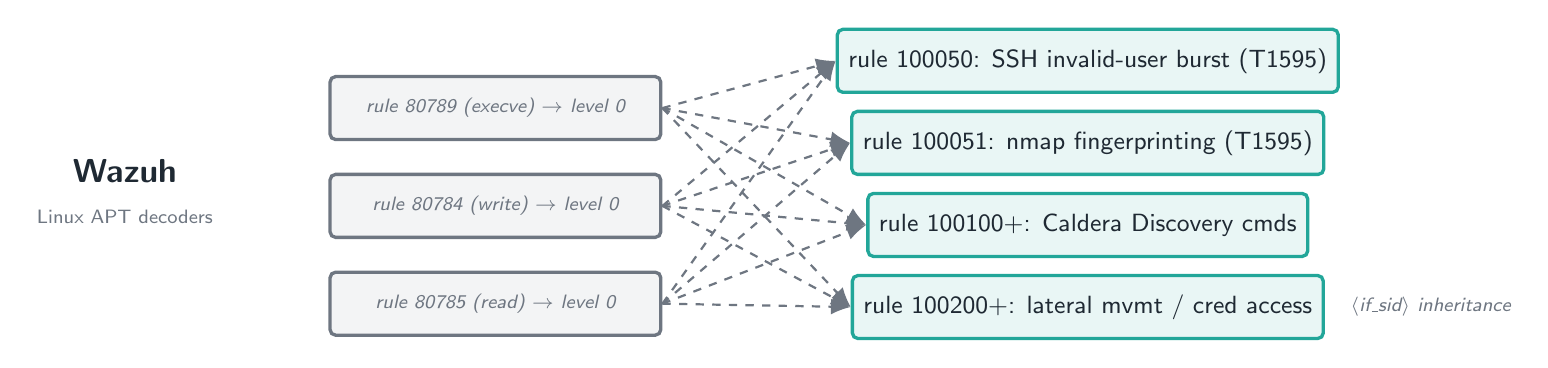
\begin{tikzpicture}[node distance=8mm,
  parent/.style={comp=strixGrey, minimum width=42mm},
  muted/.style={comp=strixGrey, fill=strixGrey!8, minimum width=42mm,
                font=\sffamily\scriptsize\itshape, text=strixGrey},
  child/.style={comp=strixGreen, minimum width=46mm},
  alert/.style={comp=strixRed, minimum width=46mm}]

\node[font=\sffamily\bfseries\large, text=strixDark] (logo) {Wazuh};
\node[font=\sffamily\scriptsize, text=strixGrey, anchor=north] at ([yshift=-1mm]logo.south) {Linux APT decoders};

% Muted parents
\node[muted, right=18mm of logo, yshift=8mm]  (p1) {rule 80789 (execve) \(\to\) level 0};
\node[muted, below=4mm of p1]                  (p2) {rule 80784 (write)  \(\to\) level 0};
\node[muted, below=4mm of p2]                  (p3) {rule 80785 (read)   \(\to\) level 0};

% Children inheriting via <if_sid>
\node[child, right=22mm of p1, yshift=6mm]   (c1) {rule 100050: SSH invalid-user burst (T1595)};
\node[child, below=2mm of c1]                (c2) {rule 100051: nmap fingerprinting (T1595)};
\node[child, below=2mm of c2]                (c3) {rule 100100+: Caldera Discovery cmds};
\node[child, below=2mm of c3]                (c4) {rule 100200+: lateral mvmt / cred access};

\foreach \p in {p1,p2,p3} {
  \foreach \c in {c1,c2,c3,c4} {
    \draw[edge, dashed] (\p.east) -- (\c.west);
  }
}

\node[font=\sffamily\scriptsize\itshape, text=strixGrey, anchor=west]
  at ([xshift=2mm]c4.east) {\(\langle\)if\_sid\(\rangle\) inheritance};

\end{tikzpicture}
\end{document}
